\documentclass[12pt]{extarticle}
\usepackage{amsmath}
\usepackage{amssymb}
\usepackage{tikz, pgfplots}
\usepackage{graphicx}
\graphicspath{ {../../chap09/} }
\usepackage[top=1in, bottom=0.75in, left=0.75in, right=0.75in]{geometry}
\newcommand*{\Scale}[2][4]{\scalebox{#1}{\ensuremath{#2}}}%
\usepackage{hyperref}
\usepackage[most]{tcolorbox}
\definecolor{bg}{RGB}{255,249,227}
\setlength{\parindent}{0pt}
\usepackage{parskip}
\setlength{\parskip}{10pt} % 1ex plus 0.5ex minus 0.2ex}


\begin{document}

\title{\vspace{-5ex}Math 208 Exam 3: Review for Chapter 9}
\author{}
\date{\vspace{-5ex}}
\maketitle

\vspace{-5ex}
\section{Information}

Exam 3 is on Thursday, April 15, 2021 on your Canvas class session

\begin{table}[h]
	\begin{tabular}{lll}
		\hline
		\textbf{Section} & \textbf{Time} & \textbf{Submission Deadline}   \\ \hline
		Sec 711          & 4:45pm-5:45pm  & 6:05pm \\ \hline
		Sec 202          & 6:40pm-7:40pm	& 8:10pm  \\ \hline
	\end{tabular}
\end{table}

\subsection{I have a question about how to do a problem on this study guide}
My email and office hours are posted on canvas. I will also meet with you by appointment. Many of the problems in this study guide have already been solved, either in the homework or during the discussion sections. Both the homework solutions and the discussion notes are posted on Canvas.


\subsection{Preparing and taking the exam}
\begin{itemize}
	\item Arrive early
	\item Know how to use your calculator
	\item Have extra pencils and an eraser
	\item Answer every question (at least minimally)
	\item If you get stuck on a question, move on to the next question and come back to it later
	\item Double check answers if time allows
	\item \textbf{Show your work!}
\end{itemize}

\subsection{Topics}
\begin{itemize}
	\item Limits and limits at infinity (4-5 questions)
	\item Derivative: the 4-step process (1 questions)
	\item Differentiation properties (6 questions)
	\item Marginal analysis (1-3 questions)
\end{itemize}


\section{Limits}
\begin{align*}
	&\lim_{x\to 2} \frac{x^2-4}{x-2}	& \lim_{x\to -1}\frac{x|x+1|}{x+1}&
\end{align*}
\begin{align*}
	&f(x) =
	\begin{cases}
		x^2-1,  & x <2\\
		x+2, & x>2
	\end{cases} \\
	&\lim_{x \to 2^-} f(x)
	&\lim_{x \to 2^+} f(x)	\\
	&\lim_{x \to 2} f(x)
	&f(2)
\end{align*}
\vspace{1cm}

\begin{center}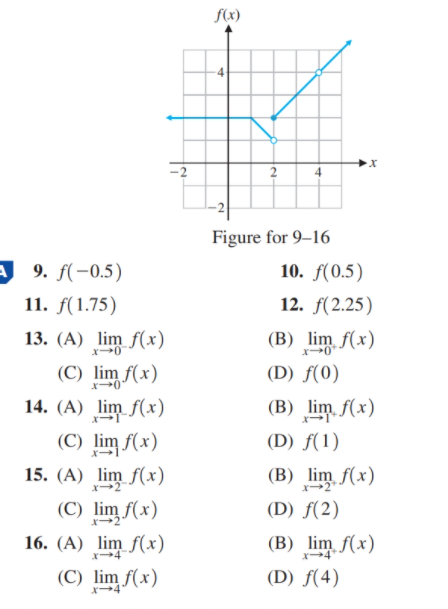
\includegraphics[width=0.6\linewidth]{9-1-9}\end{center}
\begin{center}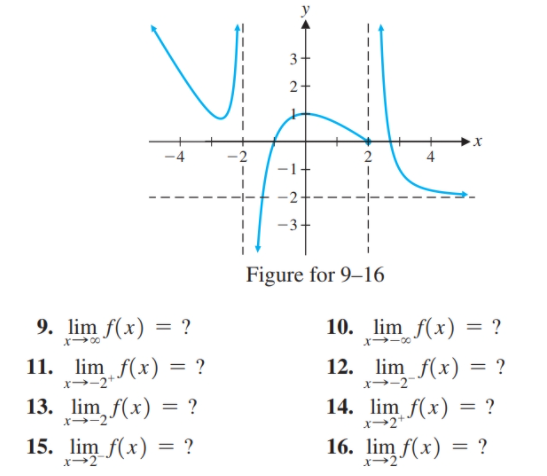
\includegraphics[width=0.6\linewidth]{9-2-8}\end{center}

For the following, find $\lim_{x\to \infty}f(x):$
\begin{center}
	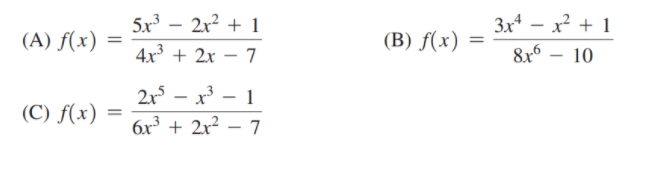
\includegraphics[width=0.8\linewidth]{9-2-11}
\end{center}
\begin{align*}
	&\lim_{x \to \infty} \frac{5+2x-3x^2}{2x^2+9} & \lim_{x \to -\infty}\frac{x+5}{x^2}& \\\\
	&\lim_{x \to -\infty} \frac{x^2-x-12}{2x^2+5x-12} & \lim_{x \to \infty}\frac{3+4x+x^2}{5-x}&
\end{align*}

Use the four step process to find the derivatives:
\begin{align*}
	&f(x) = 4x - x^2
	&f(x) = \frac{1}{x}\\
	&f(x)= 2x^2 -x &f(x)=2x^2+8
\end{align*}
\\
Use rules to find the derivatives of the following:
\begin{align*}
	&g(x)= \frac{30 + x^2 - x^3}{x^2}
	&y = 2 + 5t - 8t^3
	\\\\
	&h(w) = \frac{3w^2}{2} - \frac{7}{5\sqrt[3]{w}}
	&p=(x+1)^2 - x^3 +1
	\\\\
	&w(x) = \frac{3}{2x^2} - \frac{1}{\sqrt[5]{x^3}}
	&f(x) = 2x^2(x-4)^2 -2x
	\\\\
	&f(x) = \frac{9x^2 - 3x^3 +1}{3x^2} &y=\frac{2}{5x^4} \\\\
	&\frac{d}{dx}\left(\frac{3x^2}{2} - \frac{7}{5x^2}\right)
\end{align*}

Find the equation of the tangent line at $x=4$, where $g(x)$ is:
\begin{align*}
	g(x) = 4\sqrt{x} + 2x^2 +10
\end{align*}
Find the values of x where the tangent line is horizontal, where $f(x)$ is:
$$3x^4-6x^2-7$$

\cleardoublepage

\begin{tcolorbox}[enhanced jigsaw,colback=bg,boxrule=0pt,arc=0pt]
	\textbf{Cost, Revenue, and Profit}
	\begin{align*}
		price(x)& \text{ usually given} \tag{price} \\
		R(x)&= x* price(x) \tag{revenue} \\
		C(x)& \text{ usually given} \tag{cost} \\
		P(x)&= R(x) - C(x)\tag{profit}
	\end{align*}
Marginal Cost, Marginal Revenue, and Marginal Profit are the derivatives.
\end{tcolorbox}
\begin{tcolorbox}[enhanced jigsaw,colback=bg,boxrule=0pt,arc=0pt]
	\textbf{Exact Cost, Revenue, and Profit}
	\begin{align*}
		\text{exact cost} &= C(x+1)-C(x) \\
		\text{exact revenue} &= R(x+1) - R(x) \\
		\text{exact profit} &= P(x+1) - P(x)
	\end{align*}
\end{tcolorbox}


\begin{center}
	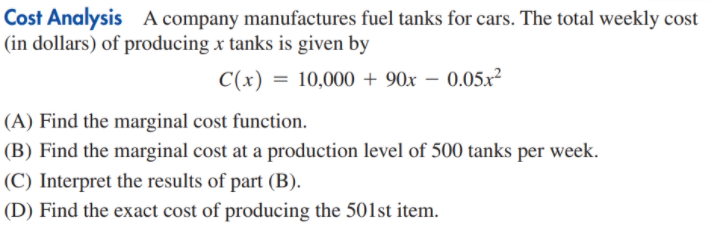
\includegraphics[width=1\linewidth]{9-7-7}
\end{center}
(E) Find the marginal cost approximation of producing the 501st item.
\\
\\
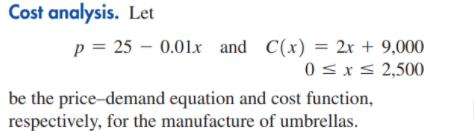
\includegraphics[width=0.75\linewidth]{9-r-1}
\\
(A) Find the marginal cost\\
(B) Find the revenue function and find the marginal revenue.\\
(C) Find the profit and marginal profit\\
(D) Evaluate the marginal profit at $x=1000, 1150, 1400$.

\cleardoublepage






\end{document}
